\documentclass[12pt]{report}

\usepackage[margin=1.0in, left=1.5in]{geometry}

\usepackage{graphicx}
\usepackage{subcaption}
\graphicspath{{./images/}}

\usepackage[
backend=biber,
style=numeric,
sorting=none
]{biblatex}
\usepackage{blindtext}
\usepackage{enumitem}
\usepackage{xcolor}
\addbibresource{references.bib}



% Title Page
\title{Robinson Observatory Telescope Refresh}
\author{Bradley Glaser, Derek McCrae, Bryan Ocbina, Justin Rudisal}

\section*{Technical Content}


\subsection*{Personal Interest}

\subsubsection*{Justin Rudisal}

My personal interest in this project is twofold with the first part being due to the subject area being space, and the second due to the project area involving a level of mechanical integration. Within my own personal experience with Internships, I have worked heavily with website development and database management. However, I have absolutely no knowledge of mechanical systems and how a computer communicates with a physical, moving part. My dream goal is working in the creative entertainment programming field, such as Universal Creative or Disney Imagineering, and so I need this basic machine programming experience to be successful in my pursuit of a career in those areas.

I also have been in love with space and space exploration for as long as I can remember, and so much so that I originally was planning on doing a double major in both Computer Science and Astronomy until I sadly realized I could not afford to pursue both. So when I heard of the senior design project that would be combining both the area of knowledge that I wish to learn more in with an area of passion that I love, I knew I had to jump on it as quickly as I could.

Other major considerations of mine for this project include the fact that it is a completely open-source undertaking. The end goal of this is to be able to document and demonstrate everything we do so that other small observatories around the world can easily duplicate our results. Projects such as that are the ones that drive my passion in programming, as well as the engineering field in general, because I fully stand behind and support anything with altruistic goals that benefits other people for the common good. I personally believe intellectual progress is achieved from the sharing of knowledge freely, and not from the selling of it for a profit.

I also want to leave a legacy behind me within my university that I have called home for the past handful of years, and that has brought so many different opportunities into my life. I want to give back to the place that has given so much to me. Being able to refresh the telescope and have my name on such a substantial undertaking is one way that I can give back and leave that legacy. I can come back years later, point at the observatory, and say "I helped repair that and bring it into the modern era". Now that is both a great resume builder, and overall achievement to be proud to talk to others about.

I remember one of my most favorite experiences from my first years at college was actually going to the observatory for "Knights Under the Stars" throughout my first few semesters, and being able to watch the telescope work and see the screen show images of our galaxy. I thought that was one of the most fascinating things ever, and it sparked an even bigger passion in astronomy in my life. Lack of time, and it's breaking, caused me to stop going as I got into my higher level classes, but that initial impression left on me caused me to instantly want to help repair the observatory when it was announced as a senior design project.



\subsection*{Broader Impacts}

Laying the foundation down for getting the telescope and observatory working again will help with both the different organizations that contract out the observatory for their own scientific pursuits, as well as enhancing its ability to reach out to students and the surrounding community with an accessible means to the stars. Even those who are not local will be able to benefit from this project due to one of our goals being to create an online public viewing platform for what the observatory is currently observing and completing. This opens it up to anyone with access to an online device to actively engage with the observatory, as well as the scientific space community at large. Our goal is to create both an online portal for the observatories sponsors to access the device, as well as crafting a learning environment for everyone.

This online outreach will also help spearhead engagement within space exploration and space overall within STEM groups both in the university as well as local elementary, middle, and high schools. Teachers will be able to pull up the current observatory pictures and developments, and will also be able to speak on weekly events that the observatory will be hosting. The overall goal is to both repair the observatory and bring it up to operating standards, as well as revamping its public outreach through new websites.

The organization that runs the observatory, Florida Space Institute, is a research group that is funded completely off of scientific grants and personal donations. By repairing this observatory for the Florida Space Institute we are helping an organization that may otherwise have a tough time affording the hiring of professionals to accomplish the intended goals. We are also helping to free up the time of those within the organization who may have had to spend their own time figuring out complicated temporary workarounds for the observatories problems instead of doing the scientific work that they want to accomplish. 

\begin{figure}
	\section*{Block Diagrams}
	\centering
	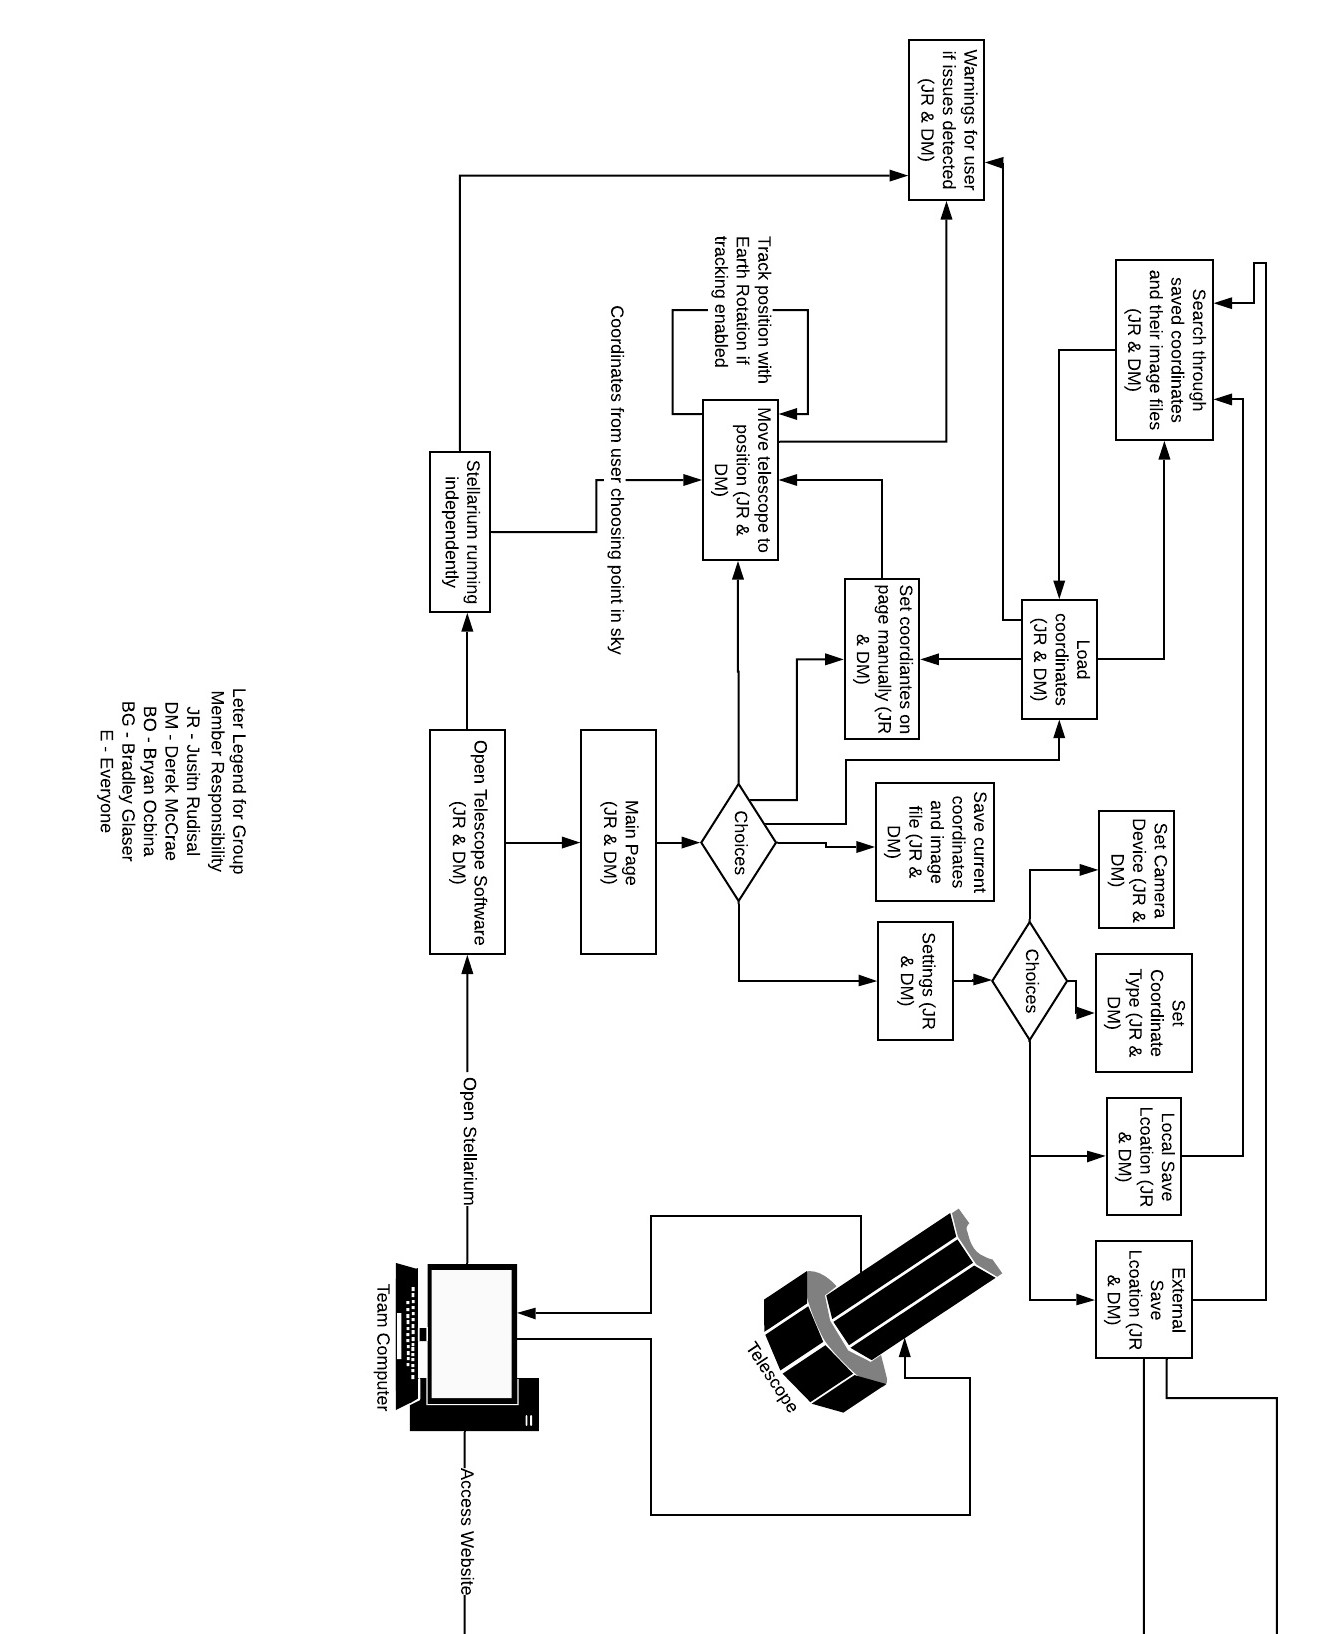
\includegraphics[height=\textheight,width=\linewidth]{blockpt2}
\end{figure}

\begin{figure}
	\centering
	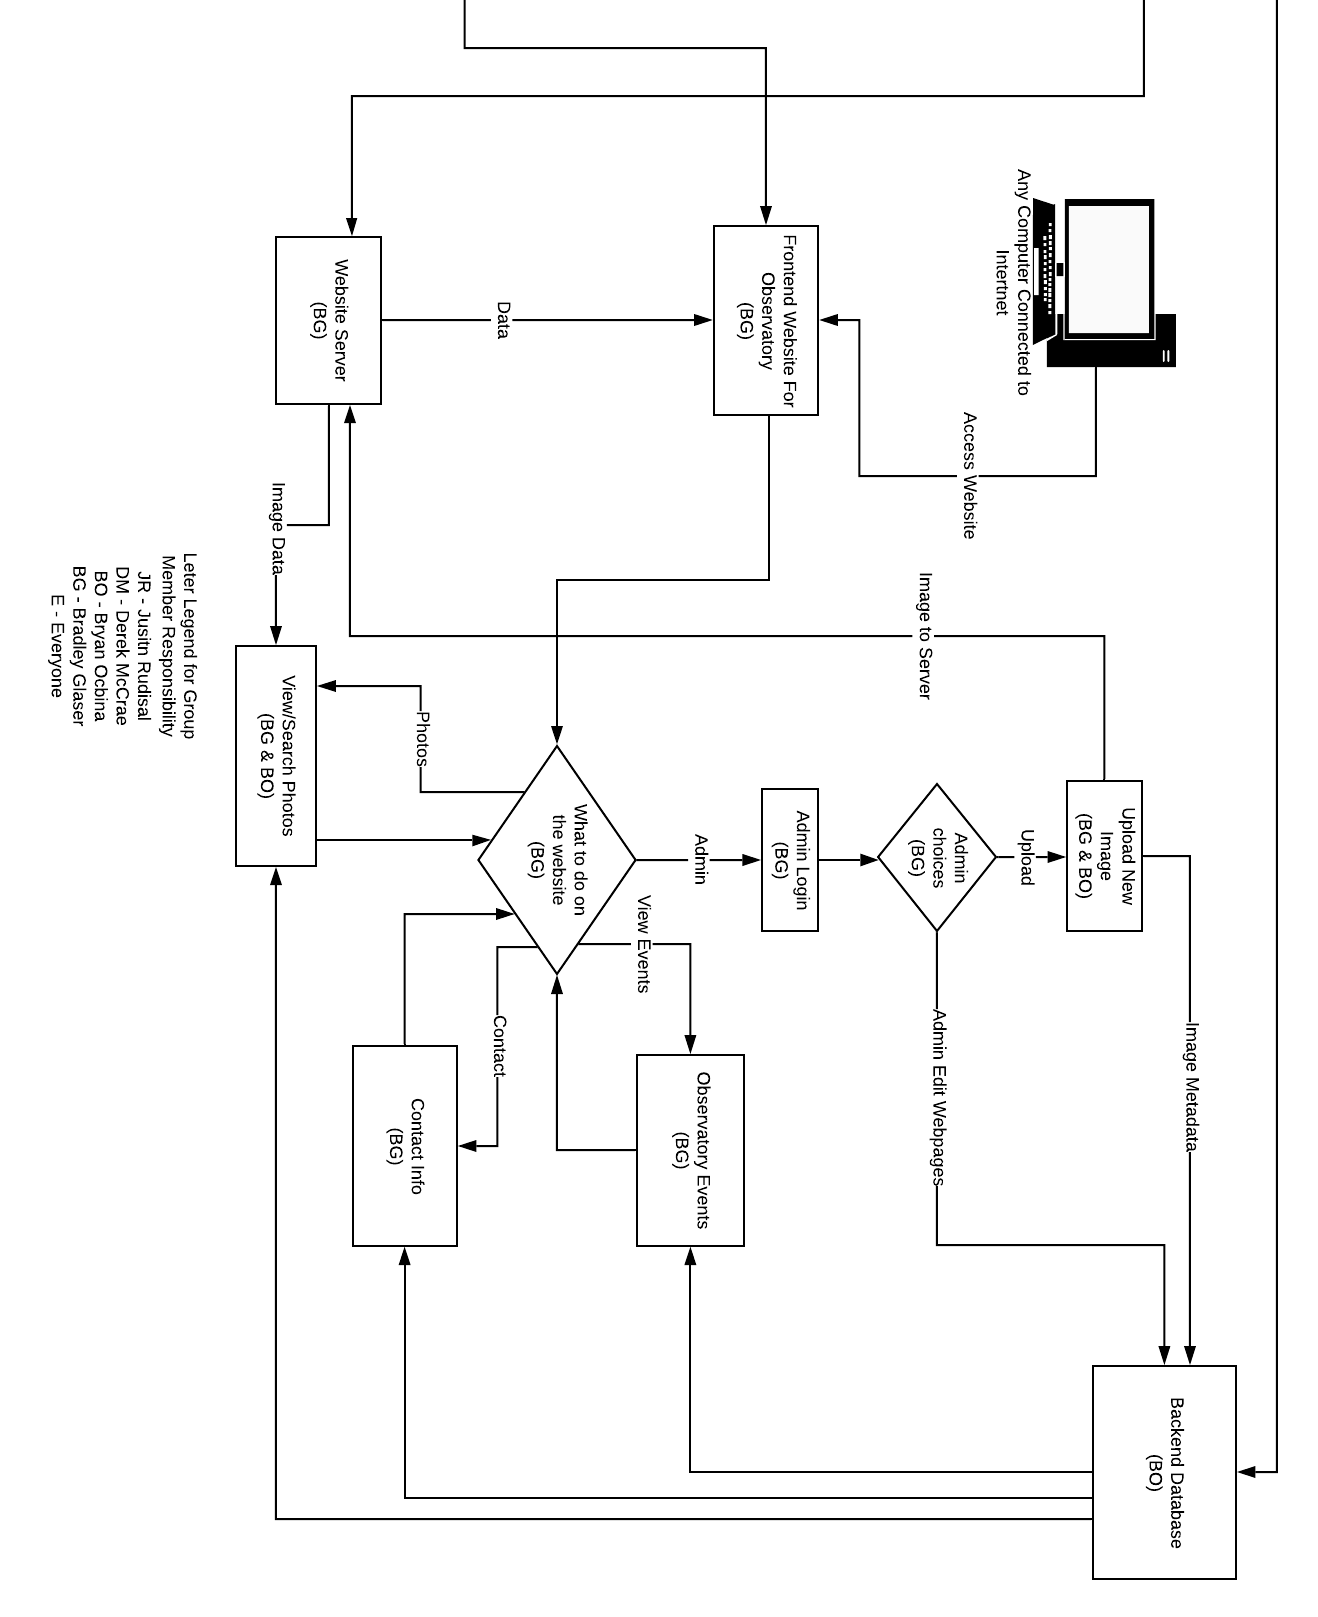
\includegraphics[height=\textheight,width=\linewidth]{blockpt1}
\end{figure}

\newpage %Page break

\begin{figure}
	\section*{Project Milestones SD1}
	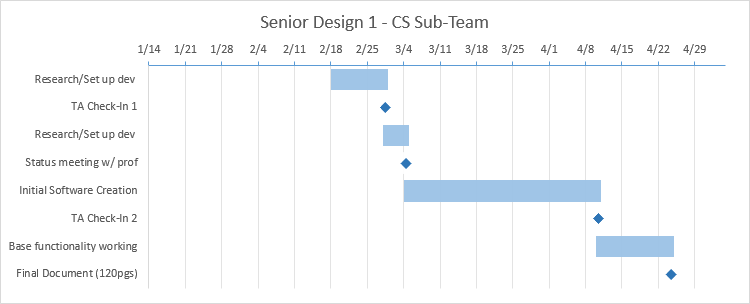
\includegraphics[width=\linewidth]{SD1Gantt}
\end{figure}

\begin{figure}
	\centering
	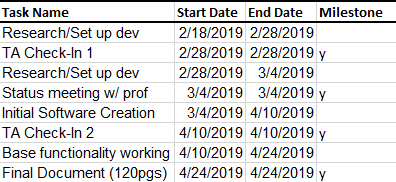
\includegraphics{SD1Dates}
\end{figure}

\clearpage

\begin{figure}
	\section*{Project Milestones SD2}
	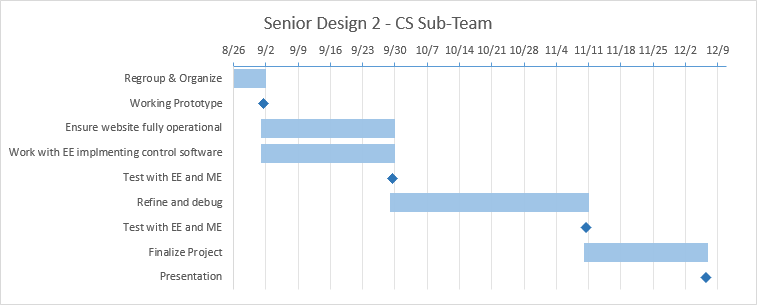
\includegraphics[width=\linewidth]{SD2Gantt}
\end{figure}

\begin{figure}
	\centering
	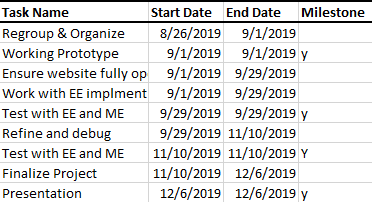
\includegraphics{SD2Dates}
\end{figure}

\clearpage



\section*{Model Telescope Control}

\subsection*{Model Telescope vs Observatory Control}

The underlying premise that drives the need for our model telescope is to replicate the control structure that the Robinson Observatory currently has in a scaled-down and testable environment. The observatory is currently controlled by a software and hardware system known as SkyX Professional, which is a commonly used product for small observatories around the globe that helps individuals get their observatory telescopes operating to their fullest extent. However, while this software is extremely useful for the observatories purposes, it is actually a hindrance for our scale model. SkyX Professional does not translate well when being adapted to small-scale custom designed telescopes. By our understanding based on documentation, as well as the physical systems currently in the Robinson observatory itself, the software has a required hardware integration to use the SkyX software for the purposes of controlling the observatory. Without this hardware, the program is nothing more than a glorified virtual observatory software for a computer with no physical controls.

To further explain, this hardware integration is not designed to be used with telescopes that have been fully planned and created from scratch. The main issue lies in that a custom telescope would have its own custom inputs and outputs based on the needs of the creator, while SkyX and its hardware is designed to integrate with well-established brands and models. The actual SkyX software and what it’s sending out and receiving form the observatory telescope is hidden behind a layer of proprietary silence, and so therein lies the need for a custom model telescope control system. We cannot use SkyX as the observatory currently uses it because we are unable to tell what the software and hardware are communicating to each other beyond our reasoning of what we think it might be sending. Assumptions can be the downfall of projects, and so we decided as an interdisciplinary team to completely circumvent SkyX and create our own software. 

\subsection*{Designing the Model Telescope Control Environment}

With the realization that we could not go the SkyX Professional route for our model telescope also came the realization that we would have to create our own custom telescope control software from scratch. Before doing any further research into what our software will do and how it will function, we first established as a team that this custom software will be open-source and easily transferable from our scale-model telescope to any real telescope. The idea behind this is that we want to be able to take our software and have senior design teams after us be able to use it as a well-defined base for repairing the Robinson Observatory. The entire thought-process behind the scale model to begin with is due to that fact that there is no currently established base, and so our team has no reference from which to repair the observatory ourselves as it stands. The hope is that with this software and model in place, future teams will have a working base form which to build off of. 

After some brainstorming and hashing around ideas, our team established that there would be little difference between our model telescope and a robot. In fact, our telescope would essentially be a controllable robot. With this in mind, we realized that we needed to establish a base software from which to do this controlling from. Taking the stance of this being a robot, we are now also free to test our designs entirely within a simulator environment to ensure our software will actually work with the physical custom model telescope.  

The following sections will discuss our plans on creating our software to control our robotic telescope. Further sections will then discuss how we plan on testing our software using a simulator environment.

\subsection*{Creating our Telescope Control Interface}

\subsubsection*{High-level Overview}

Our software will be a C++ open-sourced console application, which we will be developing in Visual Studio. We envision the application to have four base functions which are coordinate inputs to make the telescope go to a singular point in the sky, object tracking to follow an object once given it's initial position, customizable settings, and saving and loading of previously tracked objects. There is also the element of having a camera, such as a GoPro, attached to the telescope to demonstrate a visual aspect. However, this is largely dependent on the other interdisciplinary teams integrating it into the telescope and is seen as a fun stretch goal. We will design our software to include the ability to use a camera, but our project's custom telescope may not actually have one. Again, the emphasis is on the movement of the telescope and not the actual ability to view the sky. The following three sections will go into details on what each base function will entail, including mock-ups that we have created of what we envision each part will look like. Following these sections will be a further explanation of exactly how we will create this application.

\subsubsection*{Singular Point Movement vs Tracking Movement}

The main use for our model telescope will be to demonstrate the movement functionality of both our interdisciplinary teams hardware and our computer science team's software. With that being understood, the most important feature of our software is moving the telescope to focus on a single point in the sky in order to demonstrate proper movement. It will very much resemble a 'point, click, and go' method of movement. This will be accomplished by first using the aforementioned open-sourced software Stellarium to pick a point in the sky in order to pull the equatorial coordinates of that location. Once our software has those coordinates, the user will be able to decide if they want to move the telescope to this position without tracking, or move to this position and follow that point in the sky as the Earth rotates by choosing the tracking option. 

The user interface for this functionality will be very simple and to the point (Figure 1). Stellarium gives a beautiful virtual planetarium of the sky from wherever you are by taking your device's current location, or a location that the user specifies. Our software will plug into Stellarium via a toggle on the bottom taskbar of the program. When toggled on, a console application will appear showing the main screen of our software. As shown below, this will give the current equatorial coordinates of what the user has picked on the virtual planetarium. It will show empty coordinates if the user has yet to pick anything. The chosen point in the sky is denoted by a bullseye icon on the planetarium.

\begin{figure}[h]
	\centering
	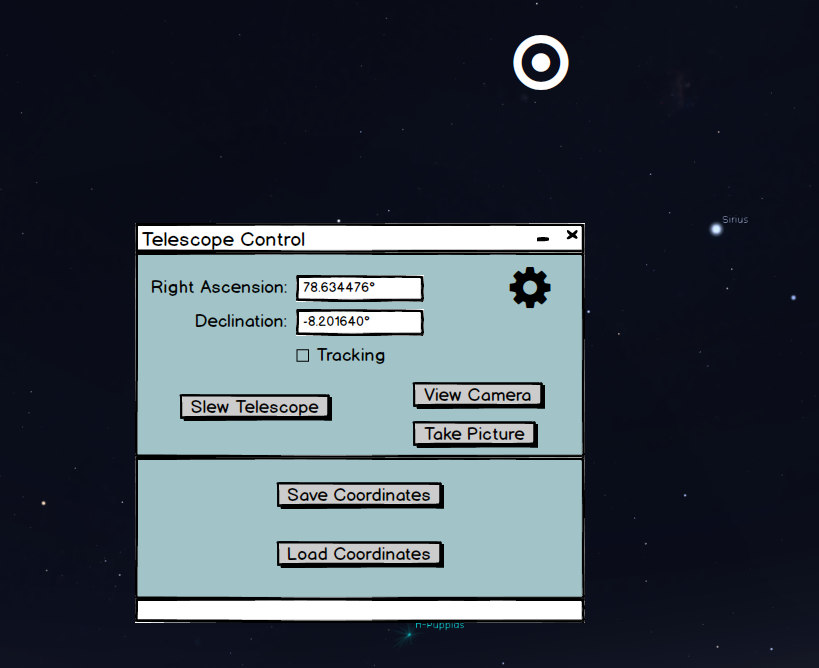
\includegraphics[width=0.85\linewidth]{MainScreen}
	\caption{Main screen of telescope control}
\end{figure}

The user will be able to move the telescope by clicking the 'Slew telescope' button when there are coordinates in the coordinate textboxes. If there is a camera currently attached, they will also be able to view whatever their current camera is visually seeing (Figure 2) as well as take a picture of the camera's view of that exact moment in time. These can be stored both externally as well as locally, and this will be explained later. 

\newpage

\begin{figure}[h]
	\centering
	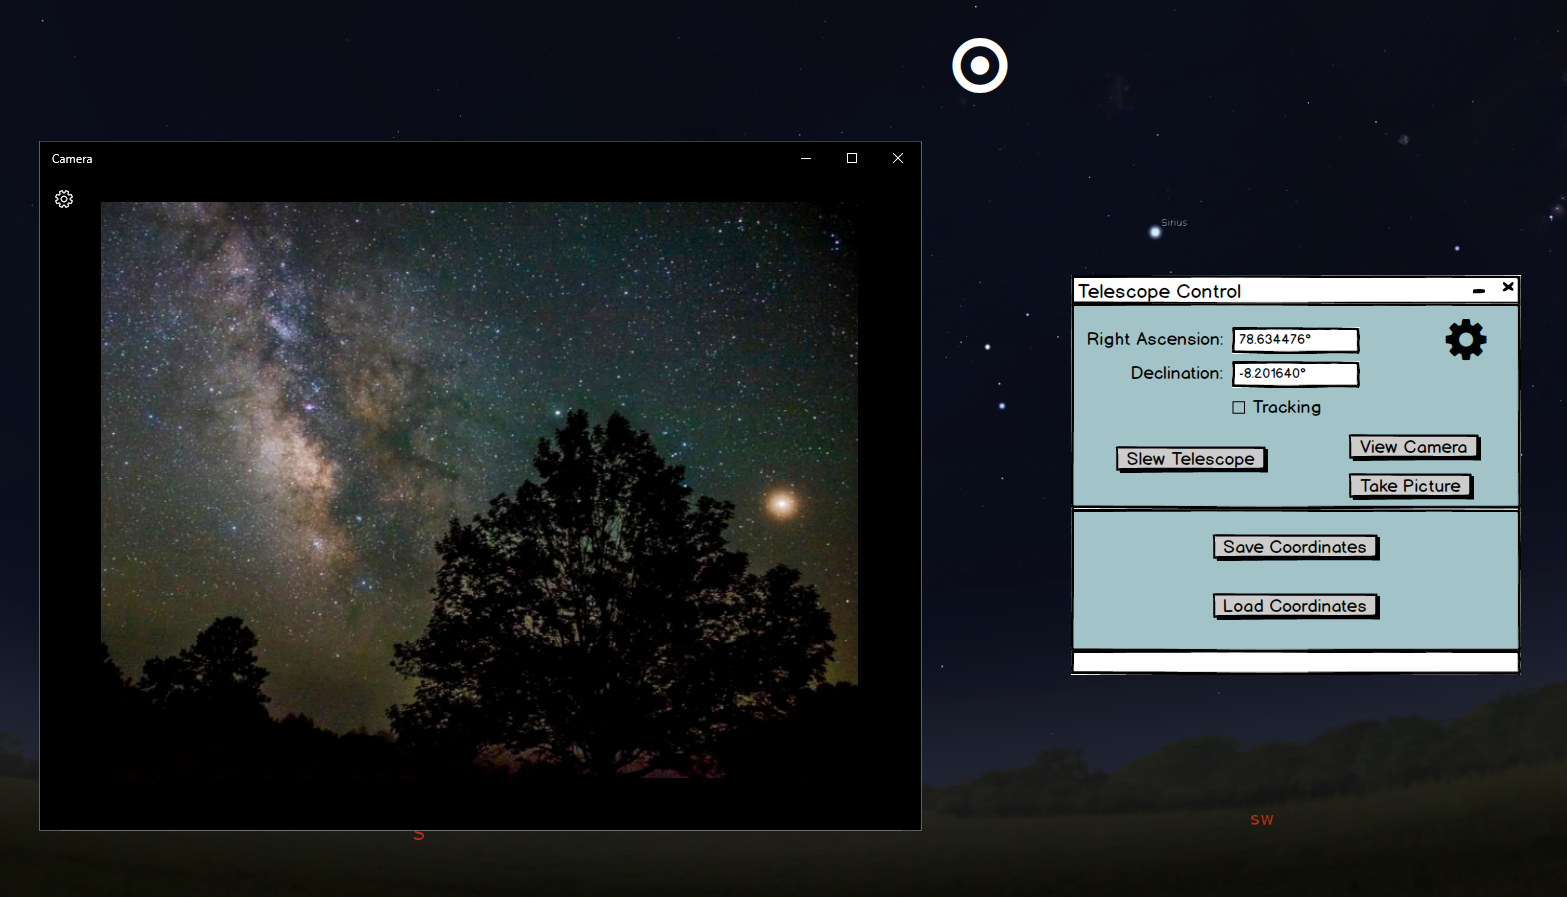
\includegraphics[width=0.90\linewidth]{MainScreenwithCameraView}
	\caption{Camera pop-up to view what the camera is currently seeing}
\end{figure}

The camera viewing application will be external of the control software, and will likely be the native camera software that comes with Windows. There will be warnings for when a camera is not detected when the user tries to use the camera options (Figure 3), or if there is no telescope detected when the user tries to move the telescope (Figure 4).

\begin{figure}[h]
	\centering
	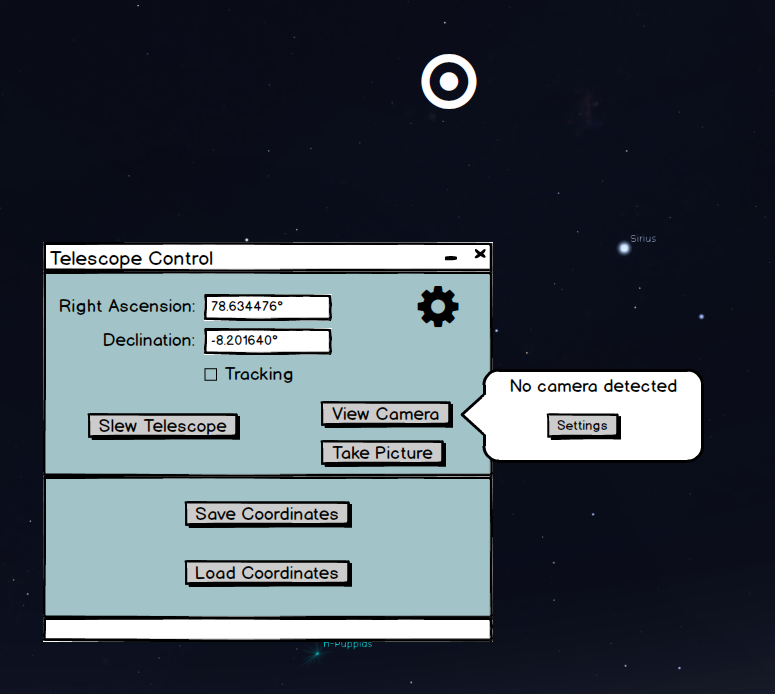
\includegraphics[width=0.70\linewidth, height=7cm]{NoCameraDetected}
	\caption{Warning that there is no camera detected}
\end{figure}

\newpage


\begin{figure}[h]
	\centering
	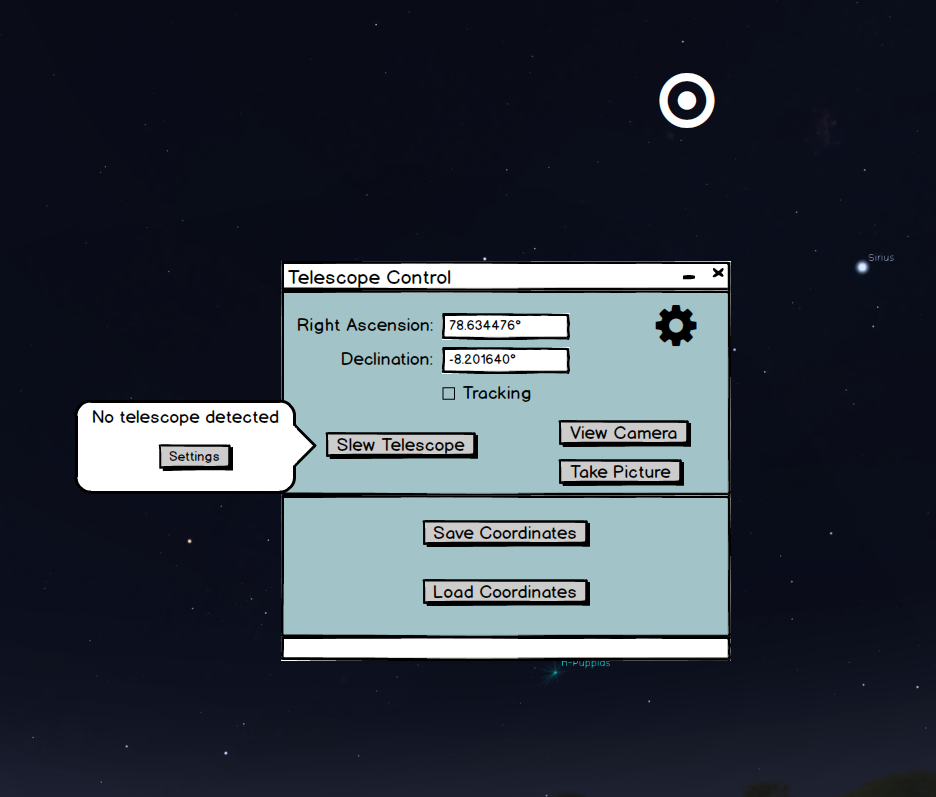
\includegraphics[width=0.70\linewidth, height=9cm]{MainScreenNoTelescope}
	\caption{Warning that there is no telescope detected}
\end{figure}

There will be fail-safes in place in case the user accidentally tries to move the telescope to an impossible position, as well as visual warnings as shown below (Figure 5). The user will have the option to override the warnings, but the telescope will stop when it reaches near a collision point, such as with the ground if the user is trying to look at a star that can currently only be soon on the opposite side of the world.

Another built-in fail-safe not necessarily shown to the user in the software is what is known as the 'Meridian Flip'. The Mechanical engineers that we are working with are designing the telescope to have a German equatorial mount. This is a type of telescope design that helps to track an object using constant speed movement on one axis that is oriented parallel to the Earth's axis of rotation. The downside to this mount is that the balancing arm, acting as a counterweight, can run into itself when tracking something that passes over the meridian line. Therefore, we will build a fail-safe that will do a 180 degree flip of the telescope when tracking across the meridian to avoid this collision.

Building this fail-safe into our software will also help further the understanding of how the Robinson Observatory's telescope works, due to it also having a German equatorial mount.

\newpage

\begin{figure}[h]
	\centering
	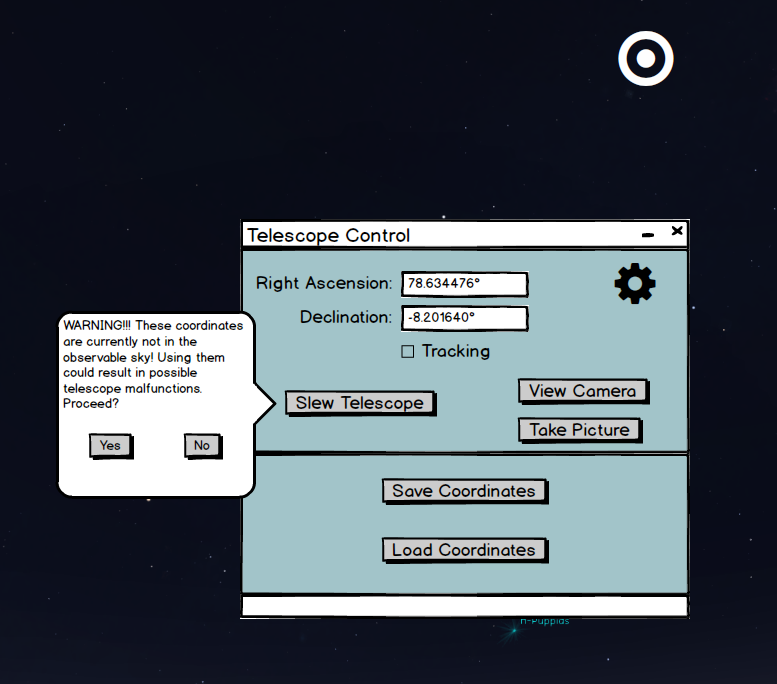
\includegraphics[width=0.80\linewidth, height=10cm]{MainScreenSlewWarning}
	\caption{Movement warning when attempting to move the telescope to an impossible position}
\end{figure}

Below these slew and camera options will finally be the saving and loading functionality as described in the next section.



\subsubsection*{Storing and Loading Previous Positions}

Other than movement, another focus of our software will be to store previous positions and movements as a list of searchable choices to then load into the telescope to move it without having to find that position manually in Stellarium's virtual planetarium again. This will be achieved by having the option to save your currently selected position along with a unique name and picture associated with the coordinates while the control console application is up and running (Figure 6). This can be done by clicking 'Save Coordinates' on the main page. Once saved, the position and chosen options are stored either locally or externally, or both, in the application to be searched for via a search user interface that can be accessed by clicking 'Load Coordinates' on the main page.

This will also remember whether or not the user decided to track the position, as well as when this particular position was saved.


\newpage
\begin{figure}[h]
	\centering
	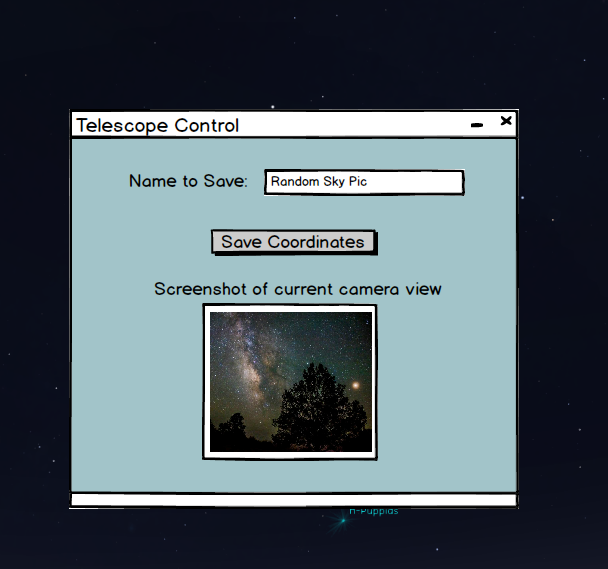
\includegraphics[width=0.60\linewidth, height=8cm]{Save}
	\caption{The save coordinates screen}
\end{figure}

This search page (Figure 7) will be dynamic in nature, searching through either both or separately files specified in a local save location and files stored in an external save location. These locations are edited in the settings, which will be further explained in the following section. As can be seen in the below figure, there will be four columns by which are self-explanatory within the figure. The unique column is the 'Picture' column, where a thumbnail of the picture related to that row's coordinate is shown. Clicking this thumbnail will cause a pop-up of the actual picture file (Figure 8). 

\begin{figure}[h]
	\centering
	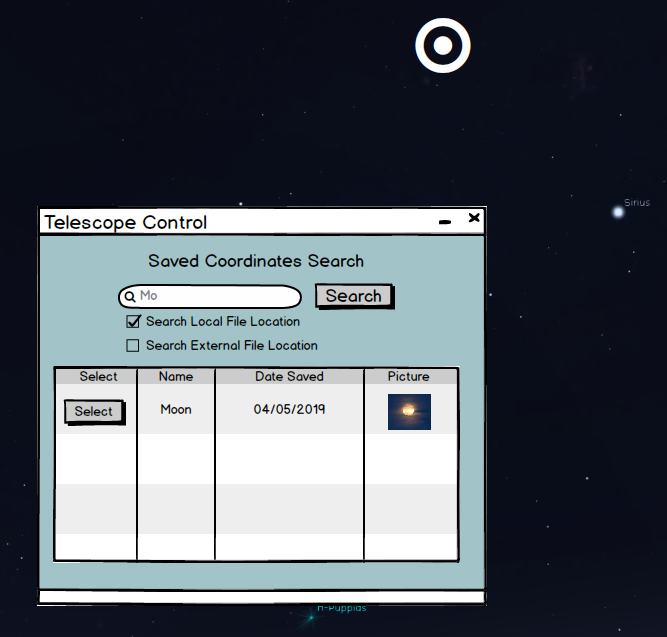
\includegraphics[width=0.55\linewidth, height=7.0cm]{SearchPage}
	\caption{The search page to load a previously saved coordinate}
\end{figure}

\newpage

\begin{figure}[h]
	\centering
	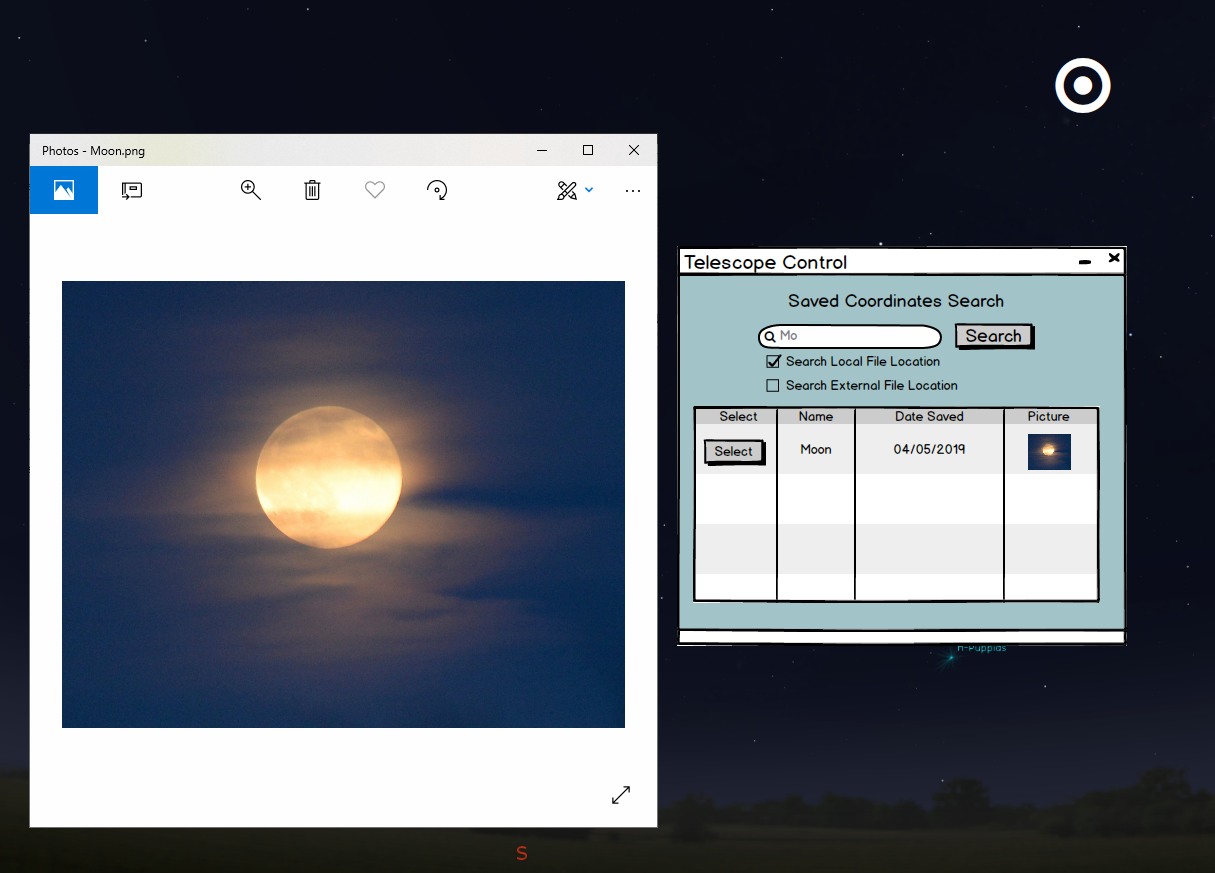
\includegraphics[width=0.65\linewidth, height=7.0cm]{SearchClickedPicture}
	\caption{By clicking the picture thumbnail, this will trigger the full-sized picture to pop up}
\end{figure}

The user can choose to load a given coordinate by clicking the select button on the chosen row, and this will bring the user back to the main page and will fill the coordinate textboxes with the saved coordinate information. However, we will have safeguards in place similar to the previously mentioned safe guards on the main page with moving the telescope. We will warn the user if they are attempting to load a coordinate that is currently not in the observable sky (Figure 9), because again this can cause possibly catastrophic issues.  

\begin{figure}[h]
	\centering
	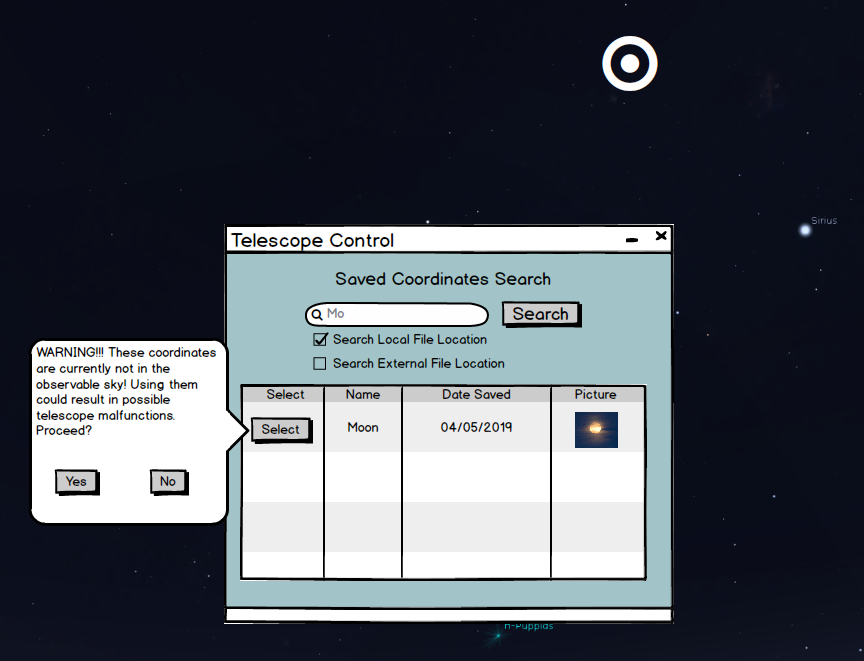
\includegraphics[width=0.65\linewidth, height=7.0cm]{SearchwithWarning}
	\caption{Warning triggered by impossible coordinates}
\end{figure}

\newpage

\subsubsection*{Setting the Settings}

The final main piece to our software is the settings page (Figure 10). This page is the customizable brains of the control software. On this page is where the user will choose from the list of detected cameras which one they would like to use as the main camera, as well as what type of format that the coordinates will have. The coordinates can have an hours-minutes-seconds, degrees-minutes-seconds, and decimal format. 

\begin{figure}[h]
	\centering
	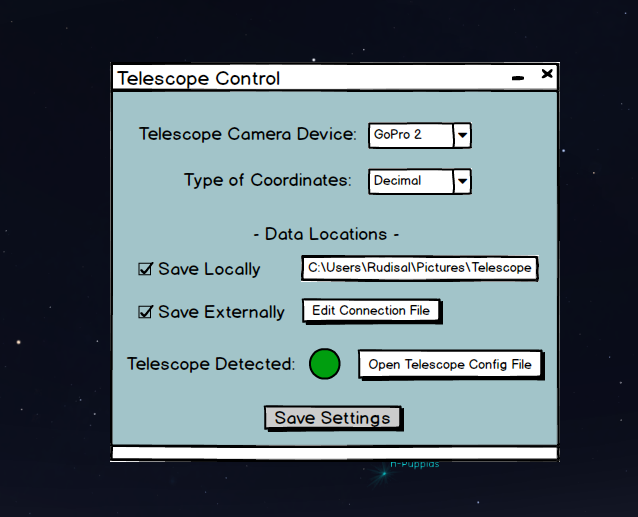
\includegraphics[width=0.75\linewidth, height=10.0cm]{Settings}
	\caption{The control software settings}
\end{figure}



Below those options is another set of options that we refer to as the 'Data Locations'. This is where the user will check whether they want to save their data that is getting stored and where that storing is happening, so long as they have one of the options checked. If both are left unchecked, then the software will assume that the user has no intention of saving any information. In terms of the 'Save Externally' option this is where the user can connect a service to the software that can take the pictures and information saved and put it on an external server, such as a website. For our project, we will set this up to communicate with the website that we are creating for the Robinson Observatory as explained later on in the paper. This 'Connection File' will require the user to have some knowledge in setting up server connections, but we will create the file with as many comments and explanations as necessary to facilitate an easy setup.

\newpage

The final part of the settings page, and arguably the most important part, is the actual telescope connection settings. Our software will be set up to automatically detect our custom telescope, but we will also create the connection file to be as easy to connect to any given telescope as we can possibly make it. There will be an indicator next to the setting that will either be green or red, dependent on whether or not a telescope is detected using the given configurated settings. Our projects main goal is to have this software work for our custom telescope, but a 'nice-to-have' goal would be to have this set up to easily connect any telescope. This will help facilitate the possibility of repairing the observatory, and could even possibly pave the way to implementing our software into actually controlling the observatory. 


\subsubsection*{Software Creation Explanation}

As mentioned previously, we will be developing this console application in C++ using Visual Studio as our IDE. We intend on making this console application as a plug-in for Stellarium, and so therefore this software will only run accurately while Stellarium is up and running.

The process that we will go about creating this software is to first establish the math associated with converting equatorial coordinates into motor rotations. The core of the physical telescope is two motors run by an Arduino, one motor controlling horizontal movement and the other controlling vertical, and these motors will rotate a certain amount of degrees based on our math. This math is further explained in the math sections later on in this paper.

The next step will be integrating that math into our visual studio console application. Once it is integrated, it is then a matter of establishing the connection to the Arduino and sending the movement commands to the motors. These commands will simply be a string containing the degree of rotation for each motor, and the Ardunio will then issue the rotation commands to the motors themselves. The Arduino and motors are the responsibility of the Electrical team. This connection is what the 'Telescope Config File' entails in the settings page of the software, and it will be the process that acts as the go-between from our software to the motors, and vice versa. 

We will then set up the auto-detection of any cameras connected to the system. We will use this auto detection to fire the camera application for the chosen camera, if one is chosen to begin with. The telescope is being designed initially to simply contain a high-grade laser to demonstrate it's accurate pointing and movement capabilities, and therefore our camera addition is not the highest priority. 

Lastly, we will develop the file that will contain the information needed for our application to communicate to an external server whenever the user specifies external data locations. This will help facilitate our telescope communicating with our website. 

\newpage

\subsection*{ROS Integration with Stand-Alone Gazebo For a Testing Environment}

\subsubsection*{Explanation for Need}

This section will explain how we intent to test our software after it is created. As mentioned previously, we will be testing the software in a simulator environment before we use it on the physical telescope itself. The actual uses for this simulator environment, as well as how we installed and set it all up, is explained in the following sections.

\subsubsection*{What is Ros?}

\begin{figure}[h]
	\centering
	
\includegraphics[width=0.50\linewidth]{melodic}
	\caption{ROS Melodic}
\end{figure}

The Robot Operating System, otherwise referred to as ROS, is a flexible framework used for the purposes of writing software for robotic systems. It is a collection of tools, libraries, and conventions that aim to simplify the task of creating complex and robust robot behavior across a wide variety of robotic platforms.\cite{ROSDescription} It is commonly used in conjunction with Python and C++, and for our purposes we will be programming in C++. Furthermore, ROS is home to a large community of user-contributed packages that adds a lot of value to integrating ROS into our core systems. Why reinvent the wheel and rediscover wood when we can instead invent a brand new cart from existing pieces already put together by other people for other projects? 

The core of ROS is licensed under the standard three-clause BSD license. This is a very permissive open license that allows for reuse in commercial and closed source products. This works great for the purposes of our model telescope, because we wish to keep our creation entirely open-sourced. While the core parts of ROS are specified as being licensed under the BSD license, other licenses are commonly used in the user-contributed community packages such as the Apache 2.0 license, the GPL license, the MIT license, and even proprietary licenses. For the sake of our aforementioned open-source goal, our team will avoid any community packages that state the use of proprietary licenses. Every user-contributed package is required to explicitly state what kind of licensing it uses, and so this should not be an issue for our team. 

\subsubsection*{What is Gazebo?}

\begin{figure}[h]
	\centering
	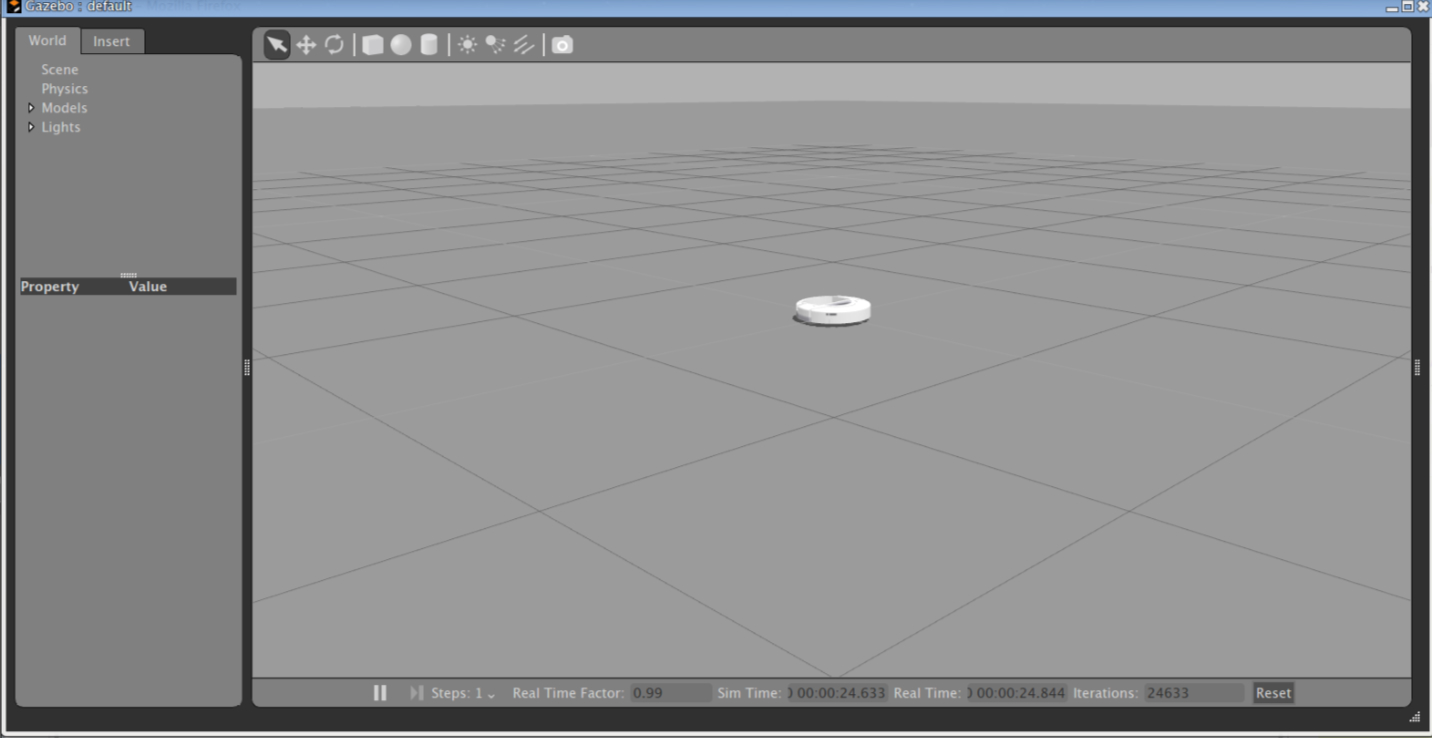
\includegraphics[width=0.90\linewidth]{gazebo}
	\caption{Example of Gazebo environment}
\end{figure}

Gazebo is a 3D dynamic simulator with the ability to accurately and efficiently simulate robotic systems in complex indoor and outdoor environments. While it appears to be similar to game engine environments, the differences in Gazebo lies in its ability to offer physics simulations at a much higher degree of fidelity, a suite of sensors, and interfaces for both users and programs.\cite{GazeboDescription} Other key features of Gazebo include multiple physics engines to choose from, a vast library of robotic models and environments, as well as advantageous programmatic and graphical interfaces. This will help create a more conductive programming environment for our team so that we can feel confident in what we create. 

Using Gazebo with our project gives us the ability to rapidly test algorithms in a simulation environment, design our model telescope with the understanding that it is a robot, perform regression testing, and possibly even train our model telescope to use a basic AI system that uses realistic scenarios. To accomplish all of this, Gazebo was designed to work on Linux operating systems and it works the best on Ubuntu, which is a flavor of Linux. Thus, this will require us to install Ubuntu in order to run Gazebo. 

\newpage

\subsubsection*{Ubuntu, a flavor of Linux}
To understand what Ubuntu is and how to install it, an individual first has to understand what Linux is. Linux is an operating system for a computer environment, and that means it is a software that manages all of the hardware resources associated with your computer. Linux is just another way to manage the communication between the software and hardware of your device.\cite{LinuxExplaination} The reasons behind why people use Linux are numerous, and the following are a few of the most common reasons:
 \begin{description}[font=$\bullet$~\normalfont\scshape\color{red!50!black}]
 	\item [Zero Cost of Entry] Linux is entirely free, and you can install it on as many systems as you would like without ever encountering a software license or fee. 
 	\item [Usability] You can do everything on Linux that you are used to doing on one of the more popular operating systems such as Windows or iOS. The key difference is that Linux has actually simplified many processes, and what can be a daunting task on one operating system is just a few commands and clicks on the Linux operating system. Hour long tasks can be accomplished in minutes. 
 	\item [System Administration] Linux is known as the "set it and forget it" operating system due to how it rarely changes it's core features, which means that you can be assured that once something is set up then you almost never have to worry about it again. Often times in other operating systems, key updates can break entire programs and cause the user to have to hunt down the issues and reconfigure multiple different areas. This is not the case with Linux, and even on the rare occasion that something within the operating system may break, almost always it does not affect any other part of the system other than the specific part that broke. 
 	\item [Open Source Licensing] Linux is also known as the operating system that is "by the people, and for the people". This is because Linux is entirely open-sourced and user-run, meaning that users have the freedom to run any programs for any purposes. They also have the freedom to redistribute any amount of copies as they wish, as well as modifying anything they would like and redistributing that as well. Linux is a virtual playground of options with almost no business-related consequences. 
 \end{description}

So then we come to the question of Ubuntu and what it has to do in relation to Linux. Linux has many different versions of itself, known as flavors, which goes hand in hand with what was stated earlier about freely modifying and redistributing Linux due to it's open-sourced nature. Ubuntu is a complete Linux operating system, and it is freely available to everyone with total support from both the community as well as professionals. The initial creators of Ubuntu created a manifesto when developing their flavor of Linux, and it's premise is that software should always be available free of charge and usable by people in their local language despite any disabilities, and that people should have the freedom to customize and alter their software in whatever way they see fit.\cite{Ubuntu} Ubuntu gets its professional support from Canonical Ltd, and Canonical's business model is to provide technical support and professional services related to Ubuntu free of charge now and always. 

To now understand why both Gazebo and ROS use and take advantage of Ubuntu, we have to learn about one final puzzle piece, the Debian Project. Debian is an all-volunteer organization dedicated to developing free software and promoting the ideals of the Free Software community. \cite{Debian} Ubuntu and Debian are distinct systems but parallel in their endeavors, which makes them closely linked. One of Ubuntu's goals is to complement the Debian project. Many of Gazebo's packages are distributed using Debian systems, and so while working with Gazebo and ROS we will also be working closely with the Debian development community.

\subsubsection*{Installing Ubuntu}
While Unbuntu itself is an amazing piece of community-sourced software development, the actual installation of the operating system into a computer is another beast entirely. While it was designed to be as seamless as possible, the issues lie in the fact that most computers already have a standard operating system on them such as Windows or iOS. This brings us to one of two options, both of which are explained below:
 \begin{description}[font=$\bullet$~\normalfont\scshape\color{red!50!black}]
	\item [Removing the current operating system and replacing it with Ubuntu] At the end of the day, operating systems are no more special than any other piece of software installed onto your device. Knowing this, it is simple to grasp that you can uninstall one operating system and replace it with another. This is a good option if you are not tied into your current operating system in any fashion, such as operating system specific software and programs that are essential to your needs, and if you are alright with switching to an entirely new type of operating system user interface and commands. It is highly recommended to have all of your information that you do not want to lose on a separate drive than what your operating system lives on, so that you do not run the risk of forever erasing any of that important data.
	\item [Installing Ubuntu beside the current operating sytem with dual-boot] You can also go the route of keeping your current operating system, and choosing to also install Ubuntu alongside it so that you can choose which operating system you will be working in on system startup. While this avoids the risks of having to untie yourself from operating system specific software, this introduces a whole new slew of risks due to this method messing with the boot manager of your motherboard's Bios and other such activities. Motherboards, the brains that control our computers, do not have built-in methods of running between two separate operating systems. Therefore, part of the Ubuntu dual-boot install requires the installing of a custom boot-up user interface, known as GRUB, that will let the user pick which operating system to use. 
\end{description}

\newpage
For the sake of our development, we went the dual-boot method so that we can maintain our current system environments while also having the ability to switch to Ubuntu for the sake of our project development. In order to begin this method we first have to create a bootable USB drive with Ubuntu installed on it so that our computer can boot into that drive. To create this bootable USB drive we needed a USB writing tool, and so we went with Rufus which is a widely-used open-sourced tool for writing ISO files onto flash drives. Having installed Rufus, as well as downloading the latest version of Ubuntu from Ubuntu's official website, we then use Rufus to make our flash drive a bootable Ubuntu USB (Figure 13).





\begin{figure}[h]
	\centering
	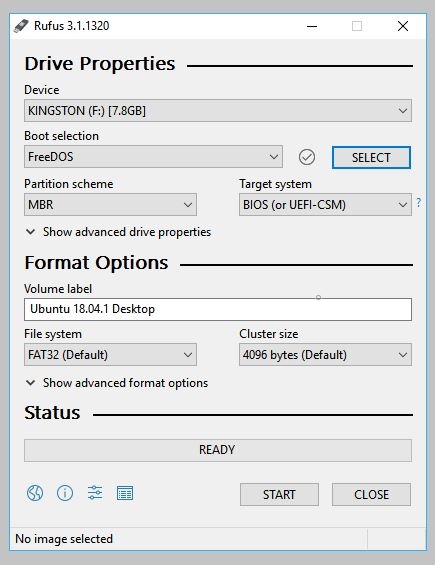
\includegraphics[width=0.50\linewidth]{rufus}
	\caption{Rufus}
\end{figure}

Once this is done, we powered down the computer and turned it back on. When first turning on, we switch the initial boot device from our normal operating system to the USB that we plugged in. This will then boot into Ubuntu where we are presented with the options to install (Figure 14). Choosing the dual-boot option on the next page will bring us through some various choices screens and account setup, and then we hit the actual installation (Figure 15). Once installed, we can now dual boot into either of our operating systems using the new GRUB menu (Figure 16).

We then have to actually set up our working environment within Ubuntu. This involves installing ROS and Gazebo and getting them up and running on our machine. The following sections will cover how to do exactly that. 

\newpage

\begin{figure}[h]
	\centering
	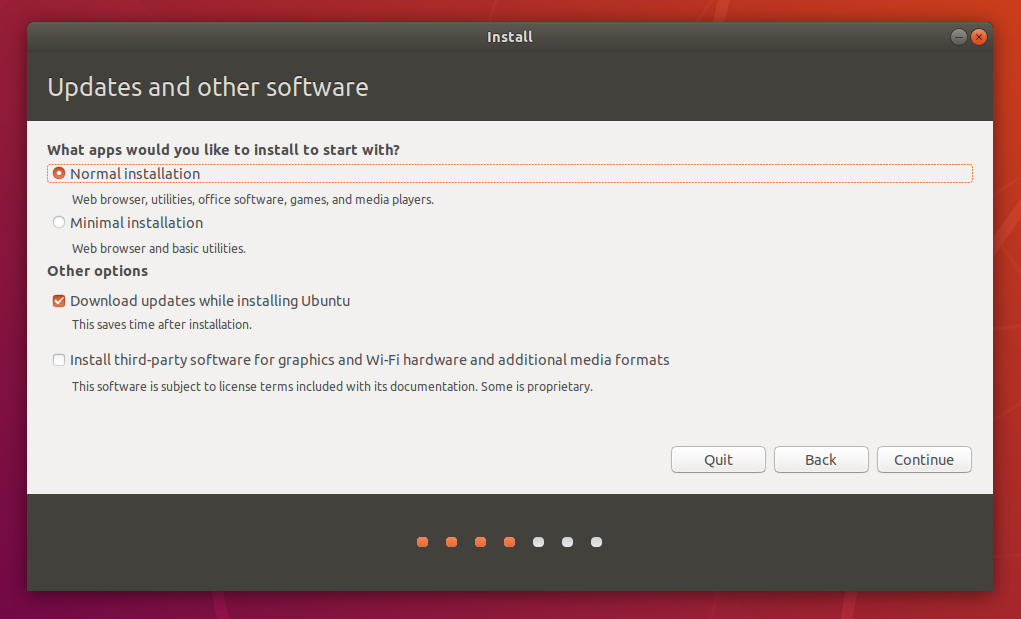
\includegraphics[width=0.50\linewidth]{install}
	\caption{Ubuntu Install Options}
\end{figure}

\begin{figure}[h]
	\centering
	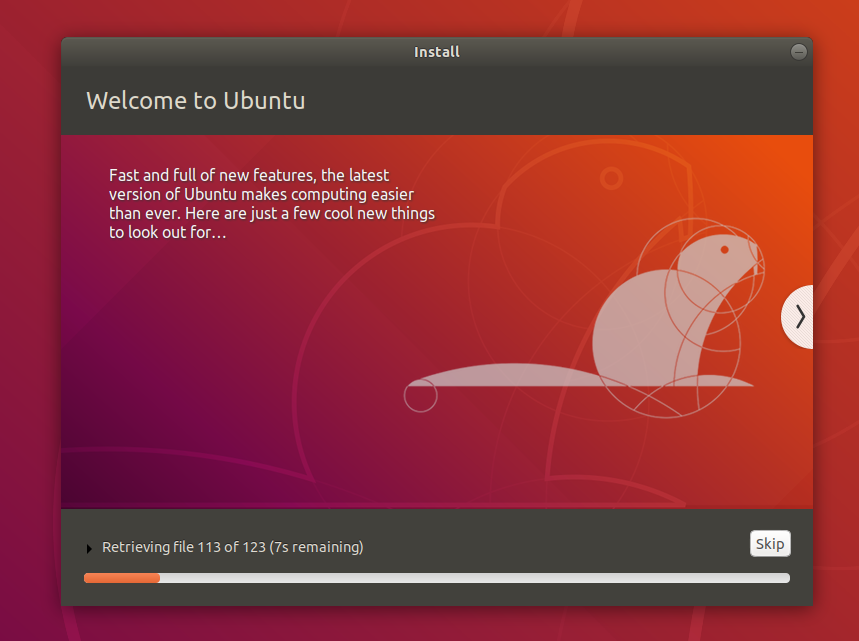
\includegraphics[width=0.50\linewidth]{installing}
	\caption{Ubuntu Installing}
\end{figure}

\begin{figure}[h]
	\centering
	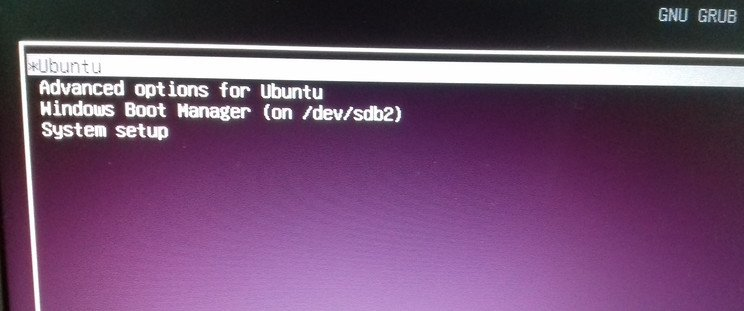
\includegraphics[width=0.42\linewidth]{dual}
	\caption{Dual-booting}
\end{figure}

\newpage

\subsubsection*{Installing Gazebo}
\indent Using Ubuntu packages, installing Gazebo is just a few simple steps. First we had to set up our computer to be able to accept software packages from 'packages.osrfoundation.org' by running the following command in the terminal:
\begin{verbatim}
sudo sh -c 'echo "deb http://packages.osrfoundation.org/gazebo/ubuntu 
`lsb_release -cs` main" > /etc/apt/sources.list.d/gazebo-latest.list'
\end{verbatim}

We then have to setup the keys and install Gazebo itself with the following terminal commands: 
\begin{verbatim}
wget http://packages.osrfoundation.org/gazebo.key -O - | sudo apt-key add -
sudo apt-get update
sudo apt-get install gazebo5
\end{verbatim}

That's it! Gazebo is successfully installed, and we cna check this by running the 'Gazebo' command on the terminal window.

\subsubsection*{Installing ROS}

 Installing ROS is an extremely similar process to installing Gazebo. In fact, that's an example of what was stated earlier about why Linux is so straightforward ot use! First we had to set up our computer to be able to accept software packages from 'packages.ros.org' by running the following command in the terminal:
 
\begin{verbatim}
sudo sh -c 'echo "deb http://packages.ros.org/ros/ubuntu $(lsb_release -sc) 
main" > /etc/apt/sources.list.d/ros-latest.list'
\end{verbatim}

We then have to setup the keys and install with the following terminal commands: 

\begin{verbatim}
sudo apt-key adv --keyserver hkp://ha.pool.sks-keyservers.net:80 --recv-key 
421C365BD9FF1F717815A3895523BAEEB01FA116
sudo apt update
sudo apt install ros-melodic-desktop-full
sudo rosdep init
rosdep update
sudo apt install python-rosinstall python-rosinstall-generator python-wstool build-essential
\end{verbatim}

There you have it, a full install of ROS. Now comes the final piece, which is integrating ROS with Gazebo.


\subsubsection*{Integrating ROS with Gazebo}
To successfully achieve a ROS integration with stand-alone Gazebo, a set of ROS packages named "gazebo ros pkgs" provided by Gazebo, provides wrappers around the stand-alone version of Gazebo.\cite{GazeboRosIntegration} They provide the necessary interfaces to simulate a robot in Gazebo using ROS messages, services and dynamic reconfiguration. 

\printbibliography[title={References}]

\end{document}
